% % \part{优化模型}
% % \chapter{全局优化}

% \documentclass[UTF8]{ctexbook}

% \ctexset{
%     part/number = \chinese{part}
% }
% \usepackage{amsmath}% ams 数学公式
% \usepackage{mathtools}% ams 数学公式
% \usepackage{amsfonts}% ams 数学字体
% \usepackage{amssymb,latexsym}% ams 数学符号与LaTeX数学符号
% \usepackage{mathrsfs}% 花式符号
% \usepackage{ntheorem}%定理、定义、证明
%   \theoremstyle{nonumberplain}
%   \theoremheaderfont{\bfseries}
%   \theorembodyfont{\normalfont}
%   \theoremsymbol{$\square$}
%   \newtheorem{Proof}{\hskip 2em 证明}
%   \newtheorem{theorem}{\hspace{2em}定理}[chapter]
%   \newtheorem{definition}{\hspace{2em}定义}[chapter] % 如果没有章, 只有节, 把上面的[chapter]改成[section]
%   \newtheorem{axiom}[definition]{\hspace{2em}公理}
%   \newtheorem{lemma}[definition]{\hspace{2em}引理}
%   \newtheorem{proposition}[definition]{\hspace{2em}命题}
%   \newtheorem{corollary}[definition]{\hspace{2em}推论}
%   \newtheorem{remark}{\hspace{2em}注}[chapter] %类似地定义其他“题头”. 这里“注”的编号与定义、定理等是分开的

% \usepackage{enumerate}%itemiz环境。\begin{enumerate}[step 1]
% \usepackage{cite}%参考文献
%     \bibliographystyle{plain}
% \usepackage{extarrows}% 带参数的箭头
% \usepackage{hyperref}% 超链接
% %\usepackage[CJKbookmarks, colorlinks, bookmarksnumbered=true,pdfstartview=FitH,linkcolor=black,citecolor=black]{hyperref}%超链接的格式设置
% \hypersetup{
%     colorlinks=false,% 去掉超链接颜色
%     pdfborder=0 0 0% 取消超链接的边框
% }
% \usepackage{graphicx}% 图片管理
% \usepackage{caption}
% \usepackage{subcaption}%并排的图各有标题
% \graphicspath{{images/}}% 设置图片搜索路径
% \usepackage{float,varwidth}% 浮动体
% \usepackage{booktabs}% 三线表
% \usepackage{fancyhdr}% 页眉设置
% \usepackage{xcolor}% 颜色宏包
% \usepackage{colortbl}% 彩色表格
% \usepackage{listings}% 代码高亮
% \usepackage{caption}% 对标题进行控制,如让\caption标题的字体缩小一号,同时数字标签使用粗体可以用:\usepackage[font=small,labelfont=bf]{caption}
% \usepackage{xfrac,upgreek}%分别是行间公式如a/b的形式(将原来的命令\frac改成\sfrac)和希腊字体的宏包的
% \usepackage{mathtools}%lgathered和rgathered环境把公式向左向右对齐
% \usepackage{tabularx}%提供自动延伸的表列,(X列格式说明符),文字过长时可以自动转行
% \usepackage{longtable}%长表格
% \usepackage{enumitem}%enumerate宏包的升级
% \usepackage{harpoon}%数学公式的矢量
% \usepackage{bookmark}%目录的书签
% \usepackage{pifont}%给数字加上圈。然后在正文输入\ding{172}~\ding{211}得到相应数字,要是要①就输入:\ding{172}②就输:\ding{173}
% \renewcommand{\headwidth}{\textwidth}%图片并排,这个要列在所有宏包的后面
% \makeatletter
% \newcommand{\rmnum}[1]{\romannumeral #1}
% \newcommand{\Rmnum}[1]{\expandafter\@slowromancap\romannumeral #1@}
% \makeatother
% \definecolor{codegreen}{rgb}{0,0.6,0}
% \definecolor{codegray}{rgb}{0.5,0.5,0.5}
% \definecolor{codepurple}{rgb}{0.58,0,0.82}
% \definecolor{backcolour}{rgb}{0.95,0.95,0.92}
% \lstset{
%     commentstyle=\color{codegreen},
%     keywordstyle=\color{magenta},
%     numberstyle=\tiny\color{codegray},
%     stringstyle=\color{codepurple},
%     basicstyle=\footnotesize,
%     breakatwhitespace=false,% 断行只在空格处
%     breaklines=true,% 自动断行
%     captionpos=b,% 标题位置
%     keepspaces=true,
%     numbers=left,
%     numbersep=5pt,
%     showspaces=false,
%     showstringspaces=false,
%     showtabs=false,% 显示
%     tabsize=2% TAB 被当作两个空格
% }
% \topmargin=0pt\oddsidemargin=0pt\evensidemargin=0pt
% \textwidth=16.5cm\textheight=23cm\raggedbottom%我这么设置是为了缩小页边距,满足有的文字无法转行
% \pagestyle{headings}%页眉为章节标题,无页脚
% \setlength{\abovecaptionskip}{4pt}
% \setlength{\belowcaptionskip}{-8pt}%图片表格的前后距离设置
% \CTEXsetup[format={\zihao{-3}\raggedright\bfseries}]{section}%设置节的格式

% \begin{document}
% \part{优化模型}
\chapter{全局优化}

\section{全局优化简介}
    \par
    在最优化刚开始的时候,我们提到过有局部极小点和全局极小点。因为全局极小点不易求解,所以我们前面都是在求局部极小点。并且提到过,如果一个问题是凸规划,则局部极小点就是全局极小点。下面,我们将来介绍非凸规划中的全局优化。全局最优化研究的是非线性目标函数在某个特征区域上全局最优点的特征和计算方法。由于目标函数通常是非凸函数,特定区域也可能不是凸集(即非凸区域),所以全局优化也称非凸优化。
    \subsection{凸集}
        \begin{definition}[凸集]
        一个集合$S\subset R^n$是凸集,即$\forall x_1,x_2\in S$,$\partial \in [0,1]$,有$\partial x^1+(1-\partial)x^2\in S$.
        \end{definition}
        \begin{definition}[凸组合]
        给定$m$个向量$x_1,x_2,\ldots,x_m \in R^n$以及$\mathop{\sum}\limits_{i=1}^{m}{\partial}_i=1,({\partial}_i \geqslant 0)$,称向量$\mathop{\sum}\limits_{i=1}^{m}{\alpha}_ix_i$为$x_1,x_2,\ldots,x_m$的凸组合.
        \end{definition}
        \begin{theorem}
        集合$S\subset R^n$是凸集,当且仅当它包含了具有有限个元素的所有凸组合,即对
        $\forall m \in {N}_+\triangleq\{1,2,\cdots\}$以及$\forall x_i(i=1,2,\cdots,m)\in S$,有$\mathop{\sum}\limits_{i=1}^{m}{\partial}_ix_i \in S$,其中:$\mathop{\sum}\limits_{i=1}^{m}{\partial}_i=1,({\partial}_i \geqslant 0)$。
        \end{theorem}
        \par
        性质:凸集关于加法、数乘、和交运算是封闭的,即$S_1+S_2,\beta S_1,S_1\cap S_2$为凸集。
        \begin{definition}[凸包]
        集合$T \subset R^n$的凸包是指所有包含$T$的凸集的交集,记为$convT = \mathop{\bigcap}\limits_{C\supseteq T}C$,其中:$C$为凸集。
        \end{definition}
        \par
        命题:若集合$S\subset R^n$是凸集,则它的闭包$S$也为凸集。
        \begin{definition}[凸锥]
        设非空集合$C \subseteq R^n$,若$\forall x \in C,\lambda >0,\lambda x \in C$,则称$C$为一个锥。此外,若$C$为凸集,该锥为凸锥。
        \end{definition}
        \par
        性质:锥关于正的数乘的运算封闭,凸锥关于加法和正的数乘运算是封闭的。一般地对于凸集$S$,集合${\mathcal{K}}(S)=\{\lambda x|\lambda >0,x\in S\}$是包含$S$的最小凸锥。
        \begin{definition}[尖锥]
        对于锥$C $,若$O \in C$,则$C$为一尖锥。
        \end{definition}
        \par
        约定:非空集合$S\subset R^n$生成的凸锥是指$S$中有限个元素非负线性组合的所有点构成的集合,记为$cone S$。特别地,若非空集合$S$是凸的,$cone S={\mathcal{K}}(S)\cup \{0\}$。
        \par
        令$\wedge(S)$表示由$S$中任何有限个点的所有凸组合的集合。可以证明$cone (S)=\wedge(S)$。这个等式反映了从"外"和"内"两个角度刻画的凸集的特征,通常互称为"对偶"。并且,如果我们用$S$内的点来表示($x\in conv(S)$)。所需要的点数不超过$d(H)$。其中,$d$是包含$S$的最小仿射子空间的维数,即集合$S$的维数$dim(S)$。
    \subsection{凸函数}
        \par
        \begin{definition}[凸函数]
        设$S\subset R^n$是非空集合,函数$f:S\to R$,若$\forall x,y\in S,\forall \lambda \in (0,1)$,有
        \begin{align*}
        f\left(\lambda x+(1-\lambda)y\right)\leqslant \lambda f(x)+(1-\lambda)f(y)
        \end{align*}
        则称$f$是$S$上的凸函数。若不等式对于$x\neq y$严格成立,则称$f$是$S$上的严格凸函数。
        \end{definition}
        \par
        易知:$-f$则$S$上的凹函数,若$-f$是$S$上的严格凸,则$f$是$S$上的严格凹函数。
        \begin{theorem}
        设$f:R^n\to R$为凸函数,则对$\forall x\in R^n$和向量$d\subset R^n/\{0\}$,函数$f$在$x$点处沿方向$d$的方向导数存在。
        \end{theorem}
        \par
        性质:\ding{172}所有凸函数$f$的集合关于凸锥组合运算是封闭的;\ding{173}函数$f$在开集$\mathop{\circ}\limits_{S}$内是连续的;\ding{174}$f$在水平集(level set)
        \begin{align*}
        L(f;\alpha) = \{x|x\in S,f(x)\leqslant \alpha\}
        \end{align*}
        和上镜图(epigraph)
        \begin{align*}
        epi(f) = \{(x,y)|x\in S,y\in R,y\geqslant f(x)\}\subset R^{n+1}
        \end{align*}
        均是凸集。
        \begin{theorem}
        设$S\in R$是非空的凸集,$f:S\to R$是凸函数,则$f$在$S$上的局部极小点也是全局极小点,且极小点的集合是凸集。
        \end{theorem}
        \begin{theorem}[水平集的有界性]
        设$S\in R$是非空的闭凸集,$f:S\to R$是二阶连续可微的凸函数。$\forall x \in S$,若$\exists m>0$,使
        \begin{align*}
        d^\mathrm{T} {\nabla}^2f(x)d \geqslant m\|d\|^2,\quad \forall x \in L(f;f(x^0)),\quad d \in R^n
        \end{align*}
        则水平集$L(f;f(x^0))$是有界的闭凸集。
        \end{theorem}
    \subsection{函数的连续性}
        \begin{definition}[下半连续]
        设$S\subset R$是非空集合,函数$f:S\to R$在$x\in S$点下半连续是指,对于$S$中任意一个收敛到$x$的点列$\{x_1,x_2,\cdots,\}$,有$f(x)=f(\mathop{\lim}\limits_{i\to \infty}x_i)\leqslant \mathop{\lim}\limits_{i\to \infty}{\inf}f(x_i)$,即$f(x)\leqslant \mathop{\lim}\limits_{y\to x}{\inf}f(y)$。
        \end{definition}
        \begin{definition}[上半连续]
        同理,$f$在$x\in S$点上半连续是指,对于$S$中任意一个收敛到$\Delta x$的点列$\{x_1,x_2,\cdots,\}$,有$f(\mathop{\lim}\limits_{i\to \infty}x_i)\geqslant \mathop{\lim}\limits_{i\to \infty}{\sup}f(x_i)$即$f(x)\geqslant \mathop{\lim}\limits_{y\to x}{\sup}f(y)$。
        \end{definition}
        \begin{definition}[连续]
        如果$f$在$x$点处上半连续又下半连续,则$f$在$x$点处连续。
        \end{definition}
        \begin{theorem}
        设$S$是$R^n$中一个非空紧集,如果$f(x)$是$S$上的下半连续函数,那么$f(x)$在$S$上至少有一个全局极小点;如果$f(x)$是$S$上的上半连续函数,则$f(x)$在$S$上至少有一个全局极大点。
        \end{theorem}
        注:若上述定理中$f$是连续的,则结论称为Weierstrass定理。
        \begin{definition}[函数的下境图]
        函数$f$的下境图(hypograh)定义为
        \begin{align*}
        hyp(f) = \{(x,y)|y\leqslant f(x),x\in S,y\in R\}\subset R^{n+1}
        \end{align*}
        \end{definition}
        \begin{definition}[函数的上境图]
        函数$f$的上境图(epigraph)定义为
        \begin{align*}
        epi(f) = \{(x,y)|y\leqslant f(x),x\in S,y\in R\}\subset R^{n+1}
        \end{align*}
        \end{definition}
        \begin{theorem}
        $f$是$S$下半连续的等价于,$\forall \partial \in R$,水平集$L(f,\partial)$是闭的,等价于上镜图$epi(f)$在$R^{n+1}$中是闭集。
        \end{theorem}
        \begin{definition}[强制]
        $f:R^n\to R$是强制的指$\mathop{\lim}\limits_{\|x\|\to \infty}f(x)=+\infty$
        \end{definition}
        \begin{theorem}
        若$f(x)$是强制的,并且下半连续,则$\mathop{\lim}\limits_{x\in R^n}f(x)$
        至少有一个全局极小点。
        \end{theorem}
        \begin{definition}[次梯度]
        一个向量$p$称为凸函数$f:S\to R$在$x\in S$的次梯度,指
        \begin{align*}
        f(y)\geqslant f(x)+p^\mathrm{T} (y-x)\quad \forall y\in S
        \end{align*}
        \end{definition}
        \begin{definition}[次微分]
        $f$在$x$点的所有次梯度的集合称为$f$在$x$点的次微分,记为$\partial f(x)$,若$\partial f(x)\neq \phi$,则$f$在$x$点次可微。
        \end{definition}
        \par
        性质:$f$在$x$点的次微分$\partial f(x)$是一个闭凸集,特别地,若$f$在$x$点是次可微的,则$\partial f(x)=\{\nabla f(x)\}$。在一般情形下,$\partial f(x)$可能是空集。
        \par
        给定一个紧凸集$S\subset R^n$,和凹函数$f:S\to R$,则$f$可以在$S$的某个极点取得全局极小点。并且,若$f$是严格凹函数,它的全局极小值只能出现在$S$的极点处。
    \subsection{凸包络}
        \par
        \begin{definition}[凸包络]
        设$S \subseteq R^n$是一个非空凸集,$f:S\to R$是下半连续函数。$f$在$S$上的凸包络是指满足如下性质的函数$F(x)$:
        \par
        \ding{172}$F(x)$在$S$上是凸的
        \par
        \ding{173}对于所有$x\in S$,$F(x)\leqslant f(x)$
        \par
        \ding{174}对于任意一个定义在$S$上的凸函数$h(x)$,$\forall x\in S,h(x)\leqslant f(x)$,则$\forall x \in S$,有$h(x)\leqslant F(x)$。
        \end{definition}
        \par
        根据凸包络的定义可以看出,凸包络是$f$在$S$上最佳一致的凸下面估计量。凸包络示意图如图(\ref{fig:凸包络示意图})所示
       \begin{figure}[H]
        \centering
        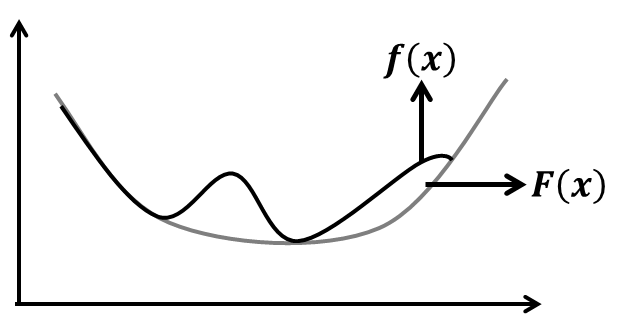
\includegraphics[width=4cm]{images/Convex_envelope.jpg}
        \caption{凸包络示意图}
        \label{fig:凸包络示意图}
        \end{figure}
        % \textcolor[rgb]{1.00,0.00,0.00}{todo:图片:凸包络示意图}
        \par
        基于凸函数这一概念,可以证明,每个凸可行域上的非凸规划问题,相伴着一个具有相同最优值的凸规划问题,即设$f:S\to R$是定义在$R^n$中的非空紧凸集$S$上的下半连续函数,考虑
        \begin{align*}
        {global}\ \mathop{\min}\limits_{x\subset C}\  f(x)
        \end{align*}
        令$F(x)$是函数$f(x)$在$S$上的凸包络,则
        \begin{align*}
        f^x={\min}\ \{ f(x)|x\in S\}={\min}\ \{F(x)|x\in S\}
        \end{align*}
        并且
        \begin{align*}
        \{ y\in S|f(y) =f^*\}\subseteq \{y\subset S|F(y)=f^*\}
        \end{align*}
        \par
        虽然在理论上我们可以解凸包络问题,但在实际中,找一个函数的凸包络,同计算它的全局极小点一样困难。
    \subsection{lipschitz函数}
        \begin{definition}[lipschitz函数]
        在$P \subseteq R^n$上的实值函数$f$称为lipschitz函数,是指$\exists L=L(f,p)>0$(L是lipschitz常数),使得$\forall x_1,x_2 \in P$,有
        \begin{align*}
        \|f(x_2)-f(x_1)\|\leqslant L\|x_2-x_1\|
        \end{align*}
        \end{definition}
        注:连续函数不一定是lipschitz函数
        \begin{definition}[局部lipschitz函数]
        $R^n$上的函数$f(x)$称为局部lipschitz函数,是指对于每个$x_0\in R^n$,存在一个以$x_0$为球心,以$\varepsilon > 0$为半径的球$B(x_0,\varepsilon)$和常数$L>0$,使得$\forall x,y\in B(x_0,\varepsilon)$,有
        \begin{align*}
        \|f(x)-f(y)\|\leqslant L\|x-y\|
        \end{align*}
        \end{definition}
        \begin{proposition}
        设$P\subset R^n$是凸集,若函数$f$在包含$P$的一个开集上连续可微,并且在$P$上具有有界梯度,则$f$在$P$上lipschitz函数,并且具有lipschitz常数
        \begin{align*}
        L={\sup}\{\nabla h(x)|x\in P\}
        \end{align*}
        \end{proposition}
        \par
        一般来说,找到上式的上界是一件困难的事情。但是,在许多使用lipschitz函数的优化技术中,集合$P$是逐次加细的矩形或单纯形。对于此类集合,可以使用自适应的方法逼近常数$L$。区间分析方法提供了一种在矩形上估计常数$L$的十分有用的技术。lipschitz函数是十分广泛的一类函数,这类函数关于许多常见的运算是封闭的。
        \begin{proposition}
        设$f,g$是紧集$P\subset R^n$上的lipschitz函数,则下面的\underline{断言}成立:
        \par
        (1)\ $f,g$的每个线性组合在$P$上是lipschitz函数;
        \par
        (2)\ ${\max}\{f,g\}$和${\min}\{f,g\}$在$P$上是lipschitz函数;
        \par
        (3)乘积$f\cdot g$在$P$上是lipschitz函数;
        \par
        (4)\ $\forall p\in[1,+\infty),(|f|^p+|g|^p)^{1/p}$在$P$上是lipschitz函数。
        \end{proposition}
    \subsection{D.C.函数}
        \par
        根据二次函数Hesse矩阵的正负特征根,可以将二次函数表示成对应正特征根的凸部分和对应负特征根的凹部分之和。事实上,许多优化问题涉及的函数都可以表示成每个凸函数之差(differences of two concexfunctions,简记为D.C.)。
        \begin{definition}[D.C.函数]
        给定凸集$x\subseteq R^n$,函数$f:x\to R$称为集合$x$上的D.C.函数是指,$f$在$x$上可以表示为如下形式
          \begin{align*}
          f(x)=p(x)-q(x)
          \end{align*}
        其中:$p,q$均是$x$上的凸函数。
        \end{definition}
        \par
        D.C.函数类十分丰富,并且其许多运算是封闭的。
        \begin{theorem}
        设$f,g$是凸集$x\subset R^n$上的D.C.函数,则下面的函数都是$x$上的D.C.函数:
          \par
          (1)\ $\lambda f+\mu g$,$\forall \lambda,\mu \in R$;
          \par
          (2)\ ${\max}\{f,g\}$和${\min}\{f,g\}$在$P$上是lipschitz函数;
          \par
          (3)\ $|f(x)|,f^{-1}(x)={\max}\{0,f(x)\}$,$f^{-1}(x)={\min}\{0,f(x)\}$;
          \par
          (4)乘积$f\cdot g$。
        \end{theorem}
        \begin{definition}[局部D.C.函数]
        一个函数$f:R^n\to R$称为局部D.C.函数(locally D.C)是指,对于每个$x_0\in R^n$,存在一个以$x_0$为球心,以$\varepsilon$为半径的球$B(x_0,\varepsilon)$,使得$f$是$B(x_0,\varepsilon)$上的D.C.函数。
        \end{definition}
        \begin{theorem}
        每个局部D.C.函数是D.C.函数。
        \end{theorem}
        \begin{theorem}
        若函数$f:R^n\to R$的二阶偏导数处处连续,则它是D.C.函数。
        \end{theorem}
        \begin{theorem}
        在紧凸集$C\subset R^n$上的每个实值连续函数都是$C$上一致收敛的D.C.函数序列的极限。
        \end{theorem}
\section{常见的全局优化模型}
    \subsection{二次规划}
        \par
        二次规划
        \begin{align*}
        &\mathop {\min}\ f(x)=\frac 12 x^\mathrm{T} Qx+ c^\mathrm{T} x\\
        &s.t.\quad x \in D
        \end{align*}
        其中:$Q\in R^{n \times n}$是一个实对称矩阵,$c\in R^n$,$D$是$R^n$中的一个多面体。若$Q$是负半定的,则$f(x)$是凹函数;若$Q$至少有一个正的和一个负的特征值(即$Q$为不定矩阵),则相应的QP为不定二次规划问题。下面,给出一些可以用凹的或者不定的二次规划模型描述的优化问题。\\
        \ding{172}线性0-1规划
        \begin{align*}
        &\mathop {\min}\  c^\mathrm{T} x\\
        &\begin{aligned}
        s.t.\quad & Ax \leqslant b\\
        \qquad &x_i\in \{0,1\}
        \end{aligned}
        \end{align*}
        令$e=(1,\ldots,1)^\mathrm{T} \in R^n$,则上述问题等价于如下的凹二次规划
        \begin{align*}
       &\mathop {\min}\  f(x)=c^\mathrm{T} x+\mu x^{-1}(e-x)\\
       &\begin{aligned}
       s.t.\quad &Ax \leqslant b\\
       & 0\leqslant x\leqslant e
       \end{aligned}
        \end{align*}
        其中:$\mu$是一个充分大的正数。\\
        \ding{173}二次0-1规划
        \begin{align*}
       \mathop {\min}\  &f(x)=c^\mathrm{T} x+ x^\mathrm{T} Qx\\
       s.t.\quad& x_i\in \{0,1\}\\
       \qquad &i=1,2,\cdots,n
        \end{align*}
        对于任意给定的实数$\mu$,令
        \begin{align*}
       &\bar{c}=c-\mu e\\
       &\bar{Q}=Q+\mu I
        \end{align*}
        注意到,对$\forall i \in \{1,2,\cdots,n\}$,当$x_i\in \{0,1\}$时,$x_i^2=x_i$,所以转化为
        \begin{align*}
       & \mathop {\min}\ \bar{f}(x)={\bar{c}}^\mathrm{T} x+  x^\mathrm{T} {\bar{Q}}x\\
       & s.t.\quad x_i\in \{0,1\}
        \end{align*}
        其中:$\bar{f}(x)=f(x)$。特别地,如果选择$\mu$,使${\bar{Q}}=Q+\mu I$为负半定,则$\bar{f}(x)$是凹的。于是约束条件可替换为$0\leqslant x \leqslant e$。\\
        \ding{174}二次指派问题(QAP)
        \par
        给定正整数$n$以及两个元素非负的$n \times n$矩阵$A=(a_{ij})$和$B=(b_{ij})$,寻找集合$\{1,2,\ldots,n\}$的一个置换$p=\left(p(1),\cdots,p(n)\right)$,使之极小化
        \begin{align*}
       C(p)=\mathop{\sum}\limits_{i=1}^n\mathop{\sum}\limits_{j=1}^na_{ij}b_{p(i)p(j)}
        \end{align*}
        上述问题等价于下面的二次0-1规划
        \begin{align*}
       &{\min}\  \mathop{\sum}\limits_{i=1}^n\mathop{\sum}\limits_{j=1}^n\mathop{\sum}\limits_{k=1}^n\mathop{\sum}\limits_{l=1}^na_{ij}b_{kl}x_{ik}x_{jl}\\
       &\begin{aligned}
       s.t.\quad &\mathop{\sum}\limits_{i=1}^nx_{ij}=1,\quad j=1,2,\cdots,n\\
        &\mathop{\sum}\limits_{j=1}^nx_{ij}=1,\quad i=1,2,\cdots,n\\
        &x_{ij}\in\{0,1\},\quad i,j=1,2,\cdots,n
       \end{aligned}
        \end{align*}
        易看出,未知元可以表示成$n^2$维向量的形式,记为$x$。
        \begin{align*}
       &\mathop {\min}\   x^\mathrm{T} Sx\\
       &s.t.\quad x \in D
        \end{align*}
        其中:$S\in R^{n^2\times n^2}$。现在,考虑如下凹二次规划
        \begin{align*}
       &\mathop {\min}\   x^\mathrm{T} Qx\\
       &s.t.\quad x \in \Omega
        \end{align*}
        其中:$S\in \alpha I$,$\alpha \geqslant \|S\|_{\infty}$,$\Omega$是满足下面条件的所有$x \in R^{n^2}$的集合
        \begin{align*}
       & \mathop{\sum}\limits_{i=1}^nx_{ij}=1\\
       & \mathop{\sum}\limits_{j=1}^nx_{ij}=1\\
       & x_{ij}\leqslant 0
        \end{align*}
    \subsection{凹极小化问题}
        \begin{align*}
       & \mathop{\min}\limits_{x}\  f(x)\\
       & \begin{aligned}
       s.t.\quad &g(x)\geqslant 0\\
       & x\in X\subset R^n
       \end{aligned}
        \end{align*}
        其中:$f,g$为非空凸开集$X$上的凹函数。
        \par
        假设该问题的可行域是一个紧的凸集,记为$D$。整数规划、双线性规划、互补性问题等都可以变换为凹极小化问题。\\
        \ding{172}双线性规划
        \begin{align*}
       & \mathop{\min}\  f(x,y)=p^\mathrm{T} x+x^\mathrm{T} Qy+q^\mathrm{T} y\\
       & s.t.\quad x\in X,y\in Y
        \end{align*}
        其中:$X,Y$分别是$R^n,R^m$上的多胞体,$p\in R^n,q\in R^m,Q\in R^{n\times m}$。令$V(X)$和$V(Y)$分别表示$X$和$Y$的顶点集。我们知道,对每一个$x\in X$,${\min}\{f(x,y)|y\in Y\}$的解可以在$Y$的一个顶点取得。于是,上述问题可表示为
        \begin{align*}
        \mathop{\min}\limits_{x\in X,y\in Y}\  f(xy)&=\mathop{\min}\limits_{x\in X}\{\mathop{\min}\limits_{y\in Y}f(x,y)\}\\
        & =\mathop{\min}\limits_{x\in X}\{\mathop{\min}\limits_{y\in {V(Y)}}f(x,y)\}=\mathop{\min}\limits_{x\in X}g(x)
        \end{align*}
        其中:$g(x)=\mathop{\min}\limits_{y\in {V(Y)}}f(x,y)=p^\mathrm{T} x+{\min}\{(q+Q^\mathrm{T} x)^\mathrm{T} y|y\in V(Y)\}$。
        \par
        因为$V(Y)$是有限的,并且对每个$y \in V(Y)$,$f(x,y)$是$x$的仿射函数,所以${\min}\{(q+Q^\mathrm{T} x)^\mathrm{T} y|y\in V(Y)\}$是有限个仿射函数的逐点最小值。因此$g(x)$是分段线性的凹函数。\\
        \ding{173}互补性问题
        \par
        一般地,给定一个集合$D\subset R^n$和函数$g,h:R^n\to R^m$,如何寻找$x\in D$,满足
        \begin{align*}
        g(x)\geqslant 0,\ h(x)\geqslant 0,\ (g(x))^\mathrm{T} h(x)=0
        \end{align*}
        的问题称为互补性问题。
        \begin{proposition}
        若上式中的函数$h$和$g$是凸集$D$上的凹函数,则上述问题有解,当且仅当下面的凹极小化问题的全局极小值为零
        \begin{align*}
       & \mathop{\min}\  f(x)=\mathop{\sum}\limits_{i=1}^n\min \{g_i(x),h_i(x)\}\\
       & s.t.\quad g(x)\geqslant 0,\ h(x)\geqslant 0
        \end{align*}
        \end{proposition}

    \subsection{D.C.规划}
        \par
        D.C.规划指如下规划问题
        \begin{align*}
        \mathop{\min}\  &f_0(x)\\
        s.t.\quad &f_i(x) \leqslant 0,i=1,2,\cdots,m\\
        & x\in X
        \end{align*}
        其中:$X$是$R^n$的闭凸子集,并且所有的函数$f_i$都是$D.C.$函数。
        \par
        典范D.C.规划形式如下
        \begin{align*}
        \mathop{\min}\  &c^\mathrm{T} x\\
        s.t.\quad & x\in D,\ g(x)\geqslant 0
        \end{align*}
        其中:$D$是$R^n$的闭凸子集,向量$c\in R^n$,$g:R^n\to R$是凸函数。\\
        \ding{172}双层线性规划
        \begin{align*}
        \mathop{\min}\  &c_1^\mathrm{T} x+d_1^\mathrm{T} y\\
        s.t.\quad & A_1x+B_1y\geqslant b^1\\
        & x\geqslant 0\\
        &y\in {\arg\min} \  d_2^\mathrm{T} y\\
        & \begin{aligned}
        s.t. \quad &A_2x+B_2y\geqslant b^2\\
        & y\geqslant 0
        \end{aligned}
        \end{align*}
        双层线性规划等价于如下典范D.C.规划
        \begin{align*}
        \mathop{\min}\  &c_1^\mathrm{T} x+d_1^\mathrm{T} y\\
        s.t.\quad & A_1x+B_1y\geqslant b^1\\
        & A_2x+B_2y\geqslant b^2\\
        & \phi(A_2x)-d_2^\mathrm{T} y\geqslant 0\\
        & x\geqslant 0,y\geqslant 0
        \end{align*}
        其中在多面体$E=\{u|u+B_2y\geqslant b^2,y \geqslant 0\}$上,函数
        \begin{align*}
        \phi(u)={\sup}\{(b^2-u)^\mathrm{T} \lambda|B_2^\mathrm{T} \lambda \leqslant d^2,\lambda \geqslant 0\}
        \end{align*}
        是下半连续的凸函数,并且$\forall u_1\geqslant u_2$,有$\phi(u_1)\leqslant \phi(u_2)$.\\
        \ding{173}双凸规划。考虑非线性规划问题
        \begin{align*}
        \mathop{\min}\limits_{x,y}\  &f(x,y)\\
        s.t.\quad & h(x,y)= 0\\
        & g(x,y)\leqslant 0\\
        & x\in X\subset R^n\\
        & y\in Y\subset R^m
        \end{align*}
        其中:$X,Y$是紧的凸集,$h(x,y),g(x,y)$分别是定义等式约束和不等式约束的向量值函数。假设所有函数$f,h,g$是连续可微的,并且满足下面的双凸条件:
        \par
        (1)对于每一个固定的$y,f(x,y)$是关于$x$的凸函数;对于每个固定的$x,f(x,y)$是关于$y$的凸函数。
        \par
        (2)对于每一个固定的$y,h(x,y)$是关于$x$的仿射函数;对于每个固定的$x,h(x,y)$是关于$y$的仿射函数。
        \par
        (3)对于每一个固定的$y,g(x,y)$是关于$x$的凸函数;对于每个固定的$x,g(x,y)$是关于$y$的凸函数。
        \par
        (4)对于每一个固定的$y$,一阶约束规格(比如Slater约束规格)成立。
        \par
        我们将原问题首先投影到$y$的空间,可以表示成双层规划形式
        \begin{align*}
        \mathop{\min}\  &f(x,y)\\
        s.t.\quad & y\in Y\\
        & x\in \bar{X}(y) \subset X\\
        & \bar{X}(y)=\mathop{\arg\min}\limits_{x\in X}f(x,y)\\
        & \begin{aligned}
        s.t. \quad &h(x,y)\geqslant 0\\
        & g(x,y)\leqslant 0
        \end{aligned}
        \end{align*}
        因为外层$f$是关于$x,y$的双凸函数,所以又称为双凸规划。
    \subsection{Lipschitz规划}
        \par
        给定一个紧集$D\subset R^n$和实值lipschitz函数$f:P\to R$,其中开集$P \supset D$
        \begin{align*}
        \mathop{\min}\  &f(x)\\
        s.t.\quad & x \in D
        \end{align*}
        称为lipschitz规划。一般地,D可以取为下列类型的集合:
        \par
        \ding{172}$n-$矩形$\{x\in R^n|a\leqslant x\leqslant b\},a\leqslant b\in R^n$;
        \par
        \ding{173}具有顶点$v_0,\cdots,v_n$的n-单纯形$[v_0,\cdots,v_n]$;
        \par
        \ding{174}$n-$矩形$\{x\in R^n|Ax\leqslant b\},a\in  R^{n\times m},b\in R^m$;
        \par
        \ding{175}$\{x|g_i(x)\leqslant 0,i=1,2,\cdots,m\}$的集合,其中$g_i$是lipschitz函数。
        \par
        下面以非线性系统来说明
        \begin{align*}
        &h_j(x)=0\quad j\in E\\
        & g_i(x)\leqslant 0\quad i\in I\\
        & x_l\leqslant x\leqslant x_u
        \end{align*}
        在上述非线性系统中,变量的个数与等式约束的个数可以不同。上述非线性系统可以变换为如下极小极大问题
        \begin{align*}
        \mathop{\min}\limits_{x}\ &\mathop{\max}\limits_{j\in E}\ |h_j(x)|\\
        s.t.\quad & g_i(x)\leqslant 0\quad i\in I\\
        &x_l\leqslant x\leqslant x_u
        \end{align*}
        如果引进非负变量$s=\mathop{\max}\limits_{j\in E}\  |h_j(x)|$。那么,极小极大问题等价于
        \begin{align*}
        \mathop{\min}\limits_{x,s}\  &s\\
        s.t.\quad & h_j(x)-s\leqslant 0\quad j\in E\\
        &-h_j(x)-s\leqslant 0\quad j\in E\\
        &g_i(x)\leqslant 0\quad i\in I\\
        &x_l\leqslant x\leqslant x_u\quad s\geqslant 0
        \end{align*}
        \par
        若$g_i,h_j$都是lipschitz函数,则上述问题就是lipschitz优化问题。当问题的全局极小值为零时,它的全局极小点$(x^*,s^*=0)$与非线性系统的解之间存在一一对应关系。除非函数$h_j$是线性的,并且函数$g_i$是凸的,上述问题通常是非凸的约束优化问题。对此,如果使用局部优化方法求解,就可能丢失问题的某些解,甚至得到非线性系统没有解的错误结论。因此,就需要正确地辨识出问题的全局最优解$(x^*,s^*)$的存在性。
\section{最优化算法}
        求解全局优化的常用算法有:\ding{172}外逼近与割平面算法;\ding{173}凹性割方法;\ding{174}分支定界法等。
        % 在实际问题中,求解…………\textcolor[rgb]{1 0 0}{todo:引入"最优化基础.docx"最后一部分。}

% \end{document}
